\documentclass[12pt,]{article}


\usepackage{baskervillef}%polskie znaki może nie

%flow chatry
\usepackage{tikz}
\usetikzlibrary{shapes.geometric, arrows}
\usepackage{amssymb}
\usepackage{float}

\title{Sprawozadanie lernicng}
\author{Tymon Łazowy}
\date{123,2123,12}


\tikzstyle{startstop} = [ellipse, rounded corners, minimum width=2cm, minimum height=1cm,text centered, draw=black,thick,fill=red!0]

\tikzstyle{io} = [trapezium,
trapezium stretches=true,
trapezium left angle=70,
trapezium right angle=110,
thick,minimum width=2cm,
minimum height=0.85cm,
text centered,
draw=black,
fill=blue!0]

\tikzstyle{process} = [rectangle,
minimum width=3cm,
minimum height=0.85cm,
text centered,
text width=3cm,draw=black,thick,fill=orange!0]

\tikzstyle{decision} = [diamond,minimum width=1cm, minimum height=1cm, text centered, draw=black, fill=green!0,thick]

\tikzstyle{arrow} = [thick,->,>=stealth]

\begin{document}
 D: a, b liczby$\in$ $\mathbb{R}$ czy są w rzeczywistym
 
 S: x podzielnść $\in$ prawda/fałsz
\begin{figure}[h]
   
    \caption{1.10 flowchart} 
    \centering  
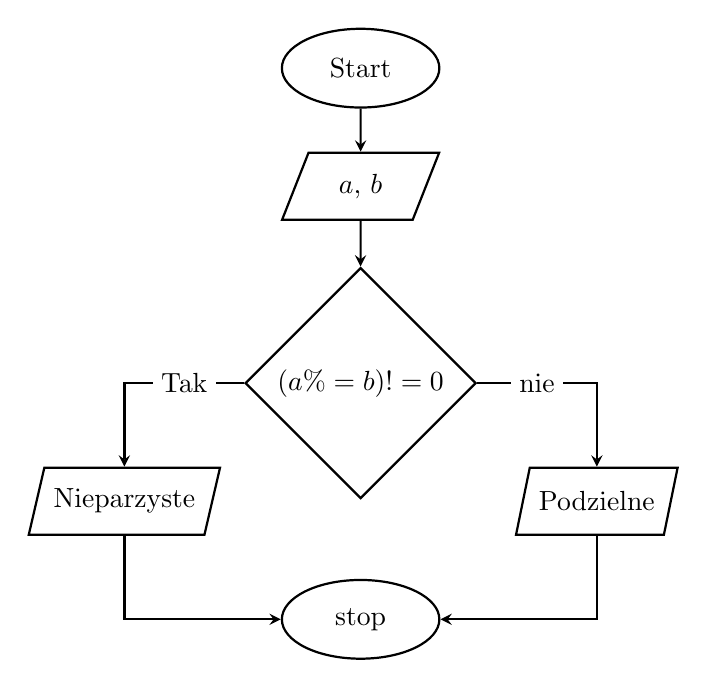
\begin{tikzpicture}[node distance=1.5cm]

\node (start) [startstop] {Start};
\node (in1) [io, below of=start,] {$a$, $b$};
\node (dec1) [decision, below of=in1,yshift=-1.cm] {$(a \%=b)!=0$};
\node (tak1) [io, left of=dec1, xshift=-1.5cm, yshift=-1.5cm] {Nieparzyste};
\node (nie1) [io, right of=dec1, xshift=1.5cm, yshift=-1.5cm] {Podzielne};
\node (stop)[startstop,below of=dec1,yshift=-1.5cm]{stop};

\draw [arrow] (start) -- (in1);
\draw [arrow] (in1) -- (dec1);
\draw[arrow] (dec1) -| (tak1) node[pos=0.25,fill=white,inner sep=3]{Tak};
\draw[arrow] (dec1) -| (nie1) node[pos=0.25,fill=white,inner sep=3]{nie};
\draw [arrow] (tak1) |- (stop);
\draw [arrow] (nie1) |- (stop);



\end{tikzpicture}
    
    \label{flow10}
\end{figure}
\end{document}